%% USEFUL LINKS:
%% -------------
%%
%% - UiO LaTeX guides:          https://www.mn.uio.no/ifi/tjenester/it/hjelp/latex/
%% - Mathematics:               https://en.wikibooks.org/wiki/LaTeX/Mathematics
%% - Physics:                   https://ctan.uib.no/macros/latex/contrib/physics/physics.pdf
%% - Basics of Tikz:            https://en.wikibooks.org/wiki/LaTeX/PGF/Tikz
%% - All the colors!            https://en.wikibooks.org/wiki/LaTeX/Colors
%% - How to make tables:        https://en.wikibooks.org/wiki/LaTeX/Tables
%% - Code listing styles:       https://en.wikibooks.org/wiki/LaTeX/Source_Code_Listings
%% - \includegraphics           https://en.wikibooks.org/wiki/LaTeX/Importing_Graphics
%% - Learn more about figures:  https://en.wikibooks.org/wiki/LaTeX/Floats,_Figures_and_Captions
%% - Automagic bibliography:    https://en.wikibooks.org/wiki/LaTeX/Bibliography_Management  (this one is kinda difficult the first time)
%%
%%                              (This document is of class "revtex4-1", the REVTeX Guide explains how the class works)
%%   REVTeX Guide:              http://www.physics.csbsju.edu/370/papers/Journal_Style_Manuals/auguide4-1.pdf
%%
%% COMPILING THE .pdf FILE IN THE LINUX IN THE TERMINAL
%% ----------------------------------------------------
%%
%% [terminal]$ pdflatex report_example.tex
%%
%% Run the command twice, always.
%%
%% When using references, footnotes, etc. you should run the following chain of commands:
%%
%% [terminal]$ pdflatex report_example.tex
%% [terminal]$ bibtex report_example
%% [terminal]$ pdflatex report_example.tex
%% [terminal]$ pdflatex report_example.tex
%%
%% This series of commands can of course be gathered into a single-line command:
%% [terminal]$ pdflatex report_example.tex && bibtex report_example.aux && pdflatex report_example.tex && pdflatex report_example.tex
%%
%% ----------------------------------------------------


\documentclass[english,notitlepage,reprint,nofootinbib]{revtex4-1}  % defines the basic parameters of the document
% For preview: skriv i terminal: latexmk -pdf -pvc filnavn
% If you want a single-column, remove "reprint"

% Allows special characters (including æøå)
\usepackage[utf8]{inputenc}
% \usepackage[english]{babel}

%% Note that you may need to download some of these packages manually, it depends on your setup.
%% I recommend downloading TeXMaker, because it includes a large library of the most common packages.

\usepackage{physics,amssymb}  % mathematical symbols (physics imports amsmath)
\include{amsmath}
\usepackage{graphicx}         % include graphics such as plots
\usepackage{xcolor}           % set colors
\usepackage{hyperref}         % automagic cross-referencing
\usepackage{listings}         % display code
\usepackage{subfigure}        % imports a lot of cool and useful figure commands
% \usepackage{float}
%\usepackage[section]{placeins}
\usepackage{algorithm}
\usepackage[noend]{algpseudocode}
\usepackage{subfigure}
\usepackage{tikz}
\usetikzlibrary{quantikz}
% defines the color of hyperref objects
% Blending two colors:  blue!80!black  =  80% blue and 20% black
\hypersetup{ % this is just my personal choice, feel free to change things
    colorlinks,
    linkcolor={red!50!black},
    citecolor={blue!50!black},
    urlcolor={blue!80!black}}


% ===========================================

\begin{document}

\title{A Brilliant Title}  % self-explanatory
\author{Erlend kristensen, Tov Tyvold, Jonathan Larsen, Sophus Gullbekk} % self-explanatory
\date{\today}                             % self-explanatory
\noaffiliation                            % ignore this, but keep it.

%This is how we create an abstract section.
\begin{abstract}
    We provide an overview of how to structure a scientific report. For concreteness, we consider the example of writing a report about an implementation of the midpoint rule of integration. For each section of the report we briefly discuss what the purpose of the given section is. We also provide examples of how to properly include equations, tables, algorithms, figures and references.
\end{abstract}
\maketitle


% ===========================================
\section{Introduction}
%
The purpose of this report template is two-fold: to communicate how to write a scientific report on a numerical topic, while simultaneously provide a concrete ``minimal working example'' of such a report. As our example topic we will look at an implementation of something rather dull and simple, namely the \textit{midpoint rule for integration}.

Throughout this example we will provide (hopefully) pedagogical commentary on report writing and structure, while at the same time present the midpoint rule for integration in a proper manner. To avoid confusion, we will from now on put pedagogical commentary in \textit{italics}. The next paragraph could have been part of the report, but we will leave it as a pedagogical comment: \textit{Writing reports, or papers, is a fundamental part of the scientific enterprise. It is vital to properly communicate precisely what has been done, what the results are and their implications. The motivation for this is to make the work understood and reproducible, so that others can both check and build on your work.}

\textit{The main purpose of the introduction section is to provide context and motivation for the work, like we have done above. It is also common --- and quite useful --- to use the last paragraph of the introduction to outline the rest of the report, to tell the reader what they should expect in the different sections. We will do this next.}

In section \ref{sec:methods} we describe the mathematical background and formulate a concrete algorithm which can be implemented in any programming language. A selection of results from a validation test are presented in section \label{sec:results}. In section \label{sec:discussion} we discuss our implementation of the algorithm in more detail, and in section \ref{sec:conclusion} we provide a short summary and outlook.

\textit{Now, since the toy example we study here is rather short and simple, our outline isn't particularly detailed. But for a report that is longer, a slightly more detailed outline might be useful.}

\section{METHODS}

\section{RESULTS}

\section{DISCUSSION}

\section{CONCLUSION}

\section{References - TEMPORARY}

\noindent
Particle Confinement in Penning Traps - An Introduction \\
Manuel Vogel \\
Springer International Publishing AG, part of Springer Nature 2018 \\
\url{https://link-springer-com.ezproxy.uio.no/book/10.1007%2F978-3-319-76264-7#authorsandaffiliationsbook}






%% USEFUL LINKS:
%% -------------
%%
%% - UiO LaTeX guides:          https://www.mn.uio.no/ifi/tjenester/it/hjelp/latex/
%% - Mathematics:               https://en.wikibooks.org/wiki/LaTeX/Mathematics
%% - Physics:                   https://ctan.uib.no/macros/latex/contrib/physics/physics.pdf
%% - Basics of Tikz:            https://en.wikibooks.org/wiki/LaTeX/PGF/Tikz
%% - All the colors!            https://en.wikibooks.org/wiki/LaTeX/Colors
%% - How to make tables:        https://en.wikibooks.org/wiki/LaTeX/Tables
%% - Code listing styles:       https://en.wikibooks.org/wiki/LaTeX/Source_Code_Listings
%% - \includegraphics           https://en.wikibooks.org/wiki/LaTeX/Importing_Graphics
%% - Learn more about figures:  https://en.wikibooks.org/wiki/LaTeX/Floats,_Figures_and_Captions
%% - Automagic bibliography:    https://en.wikibooks.org/wiki/LaTeX/Bibliography_Management  (this one is kinda difficult the first time)
%%
%%                              (This document is of class "revtex4-1", the REVTeX Guide explains how the class works)
%%   REVTeX Guide:              http://www.physics.csbsju.edu/370/papers/Journal_Style_Manuals/auguide4-1.pdf
%%
%% COMPILING THE .pdf FILE IN THE LINUX IN THE TERMINAL
%% ----------------------------------------------------
%%
%% [terminal]$ pdflatex report_example.tex
%%
%% Run the command twice, always.
%%
%% When using references, footnotes, etc. you should run the following chain of commands:
%%
%% [terminal]$ pdflatex report_example.tex
%% [terminal]$ bibtex report_example
%% [terminal]$ pdflatex report_example.tex
%% [terminal]$ pdflatex report_example.tex
%%
%% This series of commands can of course be gathered into a single-line command:
%% [terminal]$ pdflatex report_example.tex && bibtex report_example.aux && pdflatex report_example.tex && pdflatex report_example.tex
%%
%% ----------------------------------------------------


\documentclass[english,notitlepage,reprint,nofootinbib]{revtex4-1}  % defines the basic parameters of the document
% For preview: skriv i terminal: latexmk -pdf -pvc filnavn
% If you want a single-column, remove "reprint"

% Allows special characters (including æøå)
\usepackage[utf8]{inputenc}
% \usepackage[english]{babel}

%% Note that you may need to download some of these packages manually, it depends on your setup.
%% I recommend downloading TeXMaker, because it includes a large library of the most common packages.

\usepackage{physics,amssymb}  % mathematical symbols (physics imports amsmath)
\include{amsmath}
\usepackage{graphicx}         % include graphics such as plots
\usepackage{xcolor}           % set colors
\usepackage{hyperref}         % automagic cross-referencing
\usepackage{listings}         % display code
\usepackage{subfigure}        % imports a lot of cool and useful figure commands
% \usepackage{float}
%\usepackage[section]{placeins}
\usepackage{algorithm}
\usepackage[noend]{algpseudocode}
\usepackage{subfigure}
\usepackage{tikz}
\usepackage{xcolor}
\usetikzlibrary{quantikz}
% defines the color of hyperref objects
% Blending two colors:  blue!80!black  =  80% blue and 20% black
\hypersetup{ % this is just my personal choice, feel free to change things
    colorlinks,
    linkcolor={red!50!black},
    citecolor={blue!50!black},
    urlcolor={blue!80!black}}

\usepackage{algorithm}
\usepackage[noend]{algpseudocode}
\usepackage{algpseudocode}

% ===========================================

\begin{document}

\title{Penning Trap Effects}  % self-explanatory
\author{Erlend Kristensen, Tov Tyvold, Jonathan Larsen, Sophus Gullbekk} % self-explanatory
\date{\today}                             % self-explanatory
\noaffiliation                            % ignore this, but keep it.

%This is how we create an abstract section.
\begin{abstract}
    We provide an overview of how to structure a scientific report. For concreteness, we consider the example of writing a report about an implementation of the midpoint rule of integration. For each section of the report we briefly discuss what the purpose of the given section is. We also provide examples of how to properly include equations, tables, algorithms, figures and references.
\end{abstract}
\maketitle


% ===========================================

\section{Introduction}
\label{sec:INTRODUCTION}

The purpose of this report is to study the effects of a device used to store particles, the \textit{Penning trap}. Utilizing a static configuration of electric and magnetic fields to confine charged particles, the \textit{Penning trap} can be used to measure properties through precise experiments. Trapping the various particles in all three dimensions using quadrupole electrostaic field, the operations used are physically fundamental and straightforward. Throughout the analysis of an ideal \textbf{Penning trap}, we will bring forth description and functionailty for the system in time. How do we keep our particles in the device? 

\url{https://www.imperial.ac.uk/media/imperial-college/research-centres-and-groups/ion-trapping/public/PwTCP_chap1.pdf}

We start the paper in \ref{sec:INTRODUCTION} with some context beknown concerning the \textit{Penning trap} along with what we would like to gain knowledge of. In \ref{sec:METHODS} we prescribe functions that are cruicial for our trap, leading to section \ref{sec:RESULTS} where we will demonstrate and perhaps study our results. Section \ref{sec:DISCUSSION} will consist of our own interpretation of the results and a juxtaposition of the subsidiary facts. At last in \ref{sec:CONCLUSION} we will put our findings together and make a statement regarding what we wanted to know.

The \textit{Penning trap}'s invention was fueled by the realization of how the \textit{Penning gauge} by \textit{F.M. Penning} managed to shift the quadrupole field without consideration of the particles position. $REF HERE$. This advantage caught \textit{Hans Gerog Dehmlet} interest around $1955$. He managed to make a functioning prototype in $1959$, detecting axial, magntetron and cyclotron resonances, the \textit{g-factor anomaly}. Later in $1973$ \textit{Dehmlet} managed to observe, for the first time, a single trapped electron. He  recieved a \textit{Nobel Prize in Physics} in $1989$,
\\


\begin{quote}
The g-factor anomaly has now been determined by Dehmelt and his co-workers with an accuracy of a few parts in a billion, and this, together with corresponding theoretical calculations, constitutes one of the most critical tests we have of QED
\\
\end{quote}
\url{https://www.nobelprize.org/prizes/physics/1989/press-release/}
\\
In modern times, the \textit{Penning trap} technique has been further developed to create, store and cool antihydrogen. Being able to extract and use precise data from the experiment gives us the ability to further our understandings about differences between matter and antimatter as well as its profound consequences.

\url{https://alpha.web.cern.ch/motivation}
\\



\section{METHODS}
\label{sec:METHODS}

PRESENT THEORETICAL BACKGROUND
\begin{itemize}
    \item DISCUSS PHYSICS SCENARIO.
    \item EXPLAIN FORMALISM
    \item DEFINE NOTATION - CONSISTENCY 
    \item INTRODUCE FE AND RK4
\end{itemize}

WHY CAN WE TRUST THE RESULTS?

DON'T REVEAL THE RESULTS HERE 

\subsection{The Physics Scenario}

The Penning trap uses magnetic and electric fields to confine the particles. In our idealized Penning trap
the electric field is defined by \(\mathbf{E} = -\nabla \mathbf{V}\), where

\begin{align}
V(x, y, z) = \frac{V_0}{2d^2}(2z^2 - x^2 - y^2) \label{eq: electric potential}.
\end{align}

Here \(V_0\) is the voltage between \textbf{a} and \textbf{b} in fig \ref{fig: schematic} and \(d\) is the
\textit{characteristic dimension} which represents the size of the region between the electrodes where the particles are confined. As we see in fig \ref{fig: schematic} the electric field make the particles stable in the \(z\)-direction, but they are still unstable in the \(xy\)-plane. Therefore we introduce a homogeneous magnetic field \textbf{B} to stop
particles from escaping in the \(xy\)-plane. The homogenious magnetic field is given by
\(\mathbf{B} = B_0 \hat{e}_z\),
where \(B_0\) is the field strength (\(B_0 > 0\)). This will accelerate the particles towards the centre of the of the trap, giving them orbital motions. Together these fields confine the particles to a region inside the trap.

\begin{figure}[H]
    \centering
    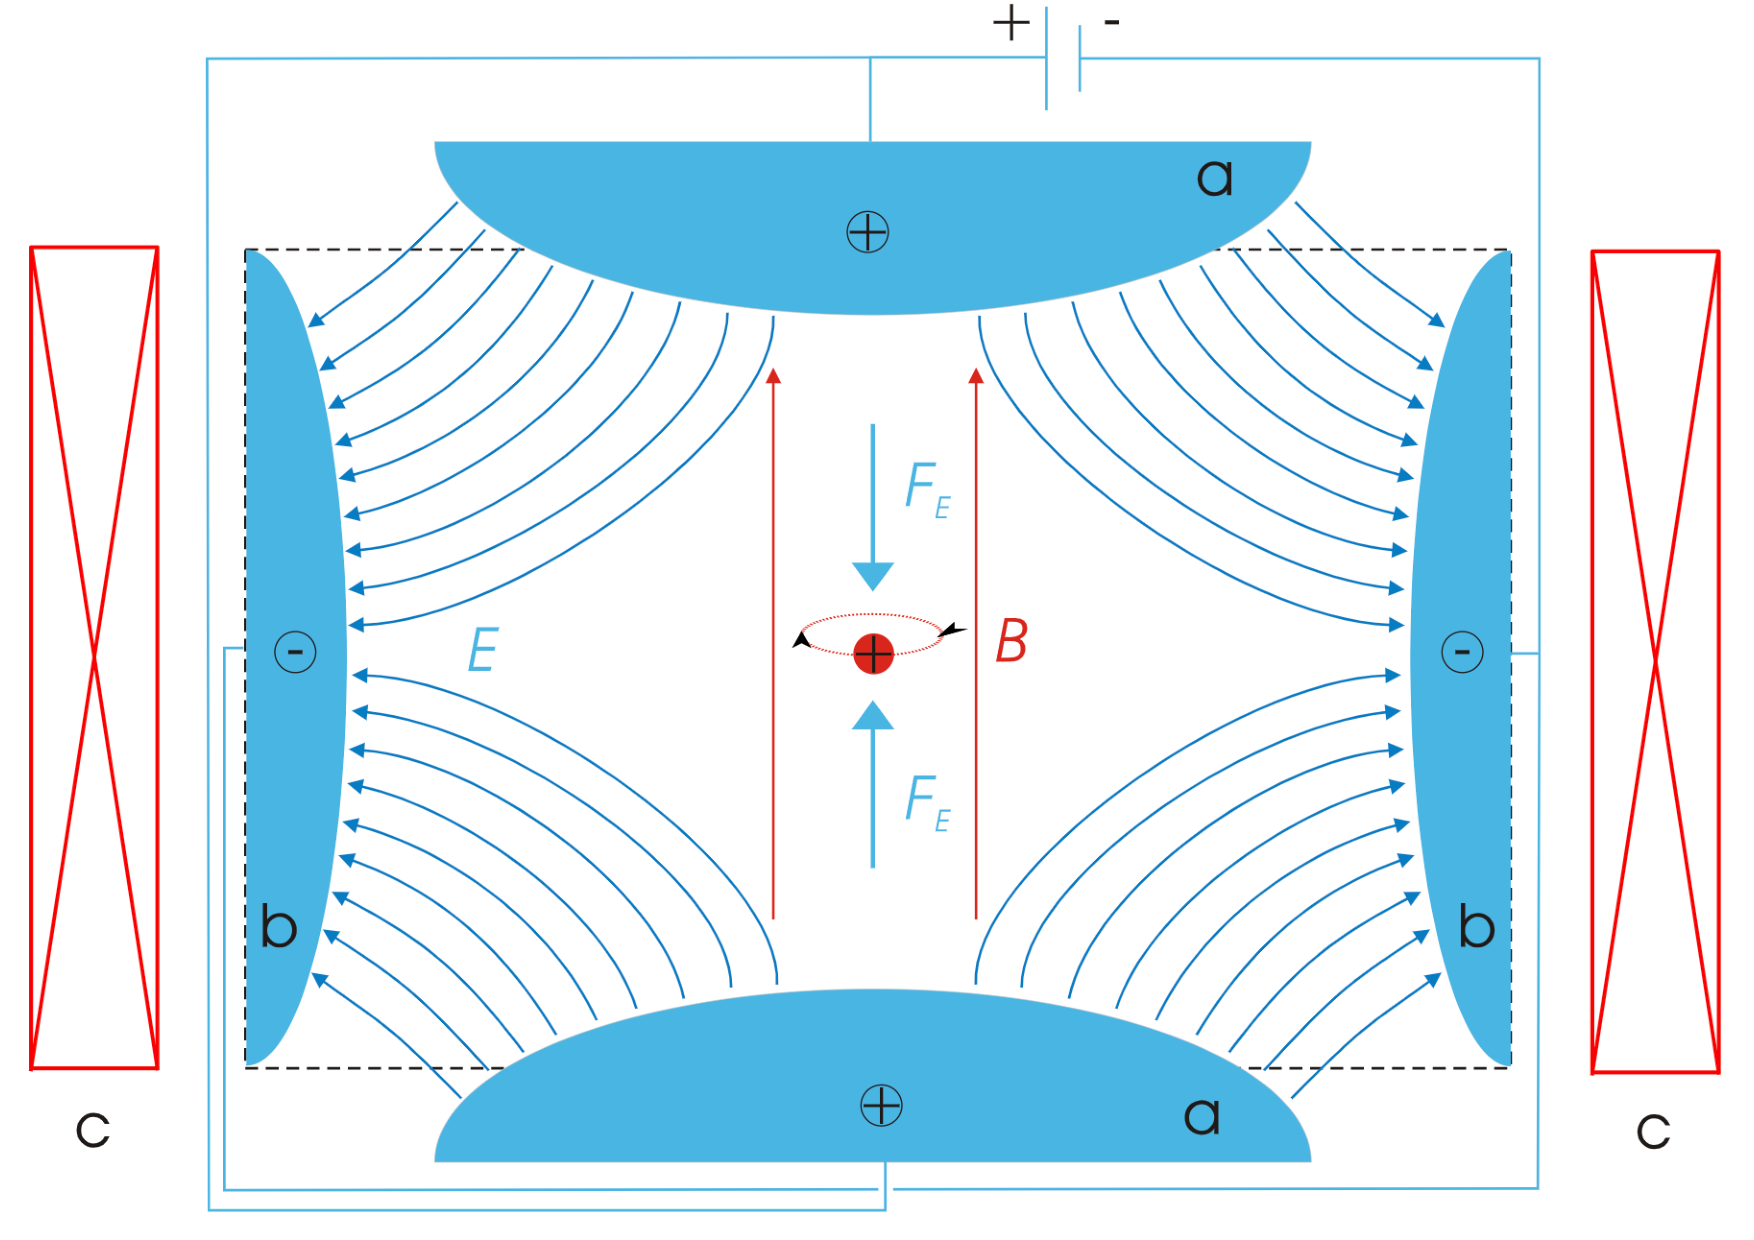
\includegraphics[width=0.5\textwidth]{schematic.pdf}
    \caption{The schematic of our Penning trap. The illustration is by Arian Kriesch and taken from 
                \href{https://en.wikipedia.org/wiki/File:Penning_Trap.svg}{Wikimedia Commons}.}
    \label{fig: schematic}
\end{figure}

To get a better understanding of how the Penning trap works we will first solve the equations of motion for a single particle in an idealized Penning trap. These describe the movement of the particle. Since there is only one particle it is possible to calculate the motion analytically, but we first need some more definitions.
\\
\\
The \textbf{Lorentz force F} is the force acting upon a particle with charge \(q\) from the electric field \textbf{E}, the magnetic field \textbf{E} and the velocity of the particle \textbf{v}. It is given by

\begin{align}
    \mathbf{F} = q\mathbf{E} + q\mathbf{V} \cross \mathbf{B}. \label{eq: lorents force}
\end{align}

Lastly we need to define the time evolution of a particle. It is given by Newtons second law,

\begin{align}
    m\Ddot{\mathbf{r}} = \sum_i \mathbf{F_i}, \label{eq: newtons 2nd}
\end{align}

Where \(m\) is the mass of the particle and \(\Ddot{\mathbf{r}}\) is the acceleration.  
Now we have enough information to derive the equations of motion of the single particle. For simplicity we assume that the charge \(q > 0\). We start with rearranging Newtons second law given in eq 
\ref{eq: newtons 2nd}, removing the summation sign since we only have one particle. 

\begin{align}
    \bf{\Ddot{r}} &= \frac{1}{m}\textbf{F} = \frac{q}{m} \left( \mathbf{E} + \mathbf{v} \times \mathbf{B} \right),
    \label{eq: newtons 2nd single particle}
\end{align}
where 
\begin{align*}
    \mathbf{E} = - \nabla V = 
    \frac{V_0}{d^2} \left(x, y, - 2z \right),
\end{align*}
\begin{align*}
    \mathbf{v} = (v_x, v_y, v_z), \quad \mathbf{B} = (0,0, B_0),
\end{align*}
\begin{align*} 
    \mathbf{v} \times \mathbf{B} = \left( v_y B_0, - v_x B_0, 0 \right).
\end{align*}
Putting everything back into eq \ref{eq: newtons 2nd single particle} we get the following equation:

\begin{align}
    \Ddot{\mathbf{r}} 
    = \omega_z^2 \left( \frac{1}{2}x, \frac{1}{2}y, -z) \right)
        + \omega_0 (v_y, v_x, 0).
\end{align}

where we define \(\omega_o \equiv \frac{q B_0}{m}\), and
\(\omega_z^2  \equiv \sqrt{\frac{2 q B_0}{m d^2}}\). 
This is equivalent to the system of equations below:

\begin{align}
    \Ddot{x}- \omega_0\cdot \Dot{y} - \frac{1}{2}\omega_z^2 \cdot x &= 0 \label{eq: x}
    \\
    \Ddot{y} + \omega_0 \cdot  \Dot{x} - \frac{1}{2}\omega_z^2 \cdot y &= 0 \label{eq: y}
    \\
    \Ddot{z} +  \omega_z^2 \cdot z &= 0 \label{eq: z}
\end{align}

These three equations Describe the trajectory of a single particle. We see that the equations representing the \(xy\)-plane are coupled, while the equation governing the axial motion is independent. This introduces some difficulty solving the first two equations, but the general solution to equation \ref{eq: z} is easy to obtain. The general solution is:

\begin{align}
    r(z) = c_1 \cos(\omega_z z) + c_2 \sin(\omega_z z)
\end{align}

{\color{purple}BURDE DET IKKE VÆRE PÅ FORMEN \(z = ...\)? 
\\
Setter inn resten av utledningen når jeg forstår det :))}
\\
\\
\\
Solving the coupled differential equations \ref{eq: x} and \ref{eq: y} is not as straight forward. First we introduce a complex function \(f(t) = x(t) + iy(t)\), such that
\(x(t) = \Re f(t)\) and \(y(t) = \Im f(t)\).
Then we define new functions for our coupled equations \ref{eq: x}
and \ref{eq: y}.

\begin{align}
    \mathcal{X}(x, \Dot{x}, \Ddot{x}) 
        \equiv \Ddot{x}- \omega_0\cdot \Dot{y} -            \frac{1}{2}\omega_z^2 \cdot x &= 0, \\
    \mathcal{Y}(y, \Dot{y}, \Ddot{y})
        \equiv \Ddot{y} + \omega_0 \cdot  \Dot{x} - \frac{1}{2}\omega_z^2 \cdot y &= 0.
\end{align}

Now it is obvious that since both \(\mathcal{X}(x, \Dot{x}, \Ddot{x}) = 0 \) and \(\mathcal{Y}(y, \Dot{y}, \Ddot{y}) = 0\)
for all \(x, y\), we must also have 
\(\mathcal{X}(x, \Dot{x}, \Ddot{x}) + i \mathcal{Y}(y, \Dot{y}, \Ddot{y}) = 0\). Lastly, since both \(x(t)\) and \(y(t)\) is at least twice differentiable we get
\(\Dot{f} = \Dot{x} +i\Dot{y}\) and 
\(\Ddot{f} = \Ddot{x} + i\Ddot{y}\).
Now we have enough information to rewrite \(\mathcal{X}\) and \(\mathcal{Y}\) as a single differential equation. 

\begin{align*}
    \mathcal{X}(x, \Dot{x}, \Ddot{x}) + i \mathcal{Y}(y, \Dot{y}, \Ddot{y}) & = 0 \\
    \Ddot{x}- \omega_0\cdot \Dot{y} -            \frac{1}{2}\omega_z^2 \cdot x
        + i \left( \Ddot{y} + \omega_0 \cdot  \Dot{x} - \frac{1}{2}\omega_z^2 \cdot y \right) & = 0 \\
    \Ddot{x} + i\Ddot{y} - \omega_0(\Dot{y} - i\Dot{x})
         + \frac{1}{2}\omega_z^2 (-x -iy) & = 0 \\
    \Ddot{f} + i\omega_0 \Dot{f} - \frac{1}{2} \omega_z^2 f
        & = 0.
\end{align*}

We have now described the coupled equations \(\mathcal{X}\) and 
\(\mathcal{Y}\) as a single differentiable equation for \(f\) given as 

\begin{align}
    \Ddot{f} + i\omega_0 \Dot{f} - \frac{1}{2} \omega_z^2 f
        & = 0. \label{eq: f(t)}
\end{align}

This allows us to calculate the general solution for \(f\), which is

\begin{align}
    f(t) = A_+ e^{-i\omega_+t} + A_- e^{-i\omega_-t},
\end{align}

where

\begin{align}
     w_{\pm} = \frac{\omega_0 \pm \sqrt{w_0^2 - 2w_z^2}}{2}
\end{align}

This function represents the movement of the particle in the \(xy\)-plane. Where there are two forces acting on our single particle. The electric field is pushing it outwards, while the magnetic field is spinning it around. The fields are moving the particle in opposing directions, and in the ideal situation they create an area of equilibrium where the particle is trapped. The next step is to calculate the necessary constraints that ensures the entrapment of the particle. This means that we need to find a solution where \(|f(t)| \leq \infty\) as \(t \to \infty\).


\subsection{Algorithms}

We have solved the equations of motion for a single particle in an idealized Penning trap, but what happens when we add more particles to the trap? When there are multiple particles in the trap, they all get coupled equations of motion. This is because each particle not only experiences the force from the electric and magnetic fields of the Penning trap, but also the Coulomb force from the other particles. 
For a set of \(n\) particles with charges \(\{q_1, \dots, q_n\}\) and masses \(\{m_1, \dots, m_n\}\) the set of equations becomes

\begin{align}
    \Ddot{x_i} - \omega_{0,i} \Dot{y}_i 
        - \frac{1}{2}\omega_{z,i}^2 x_i 
        - k_e \frac{q_i}{m_i} 
          \sum_{j\neq i}q_j \frac{x_i - x_j}{|\mathbf{r}_i - \mathbf{r}_j|^3} & = 0, \label{eq: x mult} \\ 
    \Ddot{y_i} - \omega_{0,i} \Dot{x}_i 
        - \frac{1}{2}\omega_{z,i}^2 y_i 
        - k_e \frac{q_i}{m_i} 
          \sum_{j\neq i}q_j \frac{y_i - y_j}{|\mathbf{r}_i - \mathbf{r}_j|^3} & = 0, \label{eq: y mult}\\
    \Ddot{z_i} + \omega_{z,i}^2 z_i 
        - k_e \frac{q_i}{m_i} 
          \sum_{j\neq i}q_j \frac{z_i - z_j}{|\mathbf{r}_i - \mathbf{r}_j|^3} & = 0, \label{eq: z mult}
\end{align} 

This set of coupled differential equations work for an arbitrary number of particles with particle indices \(i\) and \(j\). This time, however, it will not be possible to solve the equations analytically as we did in the previous section. This is because the Coloumb force makes the equations 
\ref{eq: x mult}, \ref{eq: y mult} and \ref{eq: z mult} non-linear. And as mentioned in the introduction: non-linear equations often don't have analytical solutions.
Therefore we need to use numerical methods. Specifically, we will consider two famous numerical methods: The trusty Forward Euler algorithm and the Runge-Kutta method. 

{\color{purple} MENTION IN THE INTRODUCTION THAT THE EQUATIONS ARE NON-LINEAR AND THEREFORE NEED NUMERICAL METHODS TO BE SOLVED.}


Both algorithms derive from the Taylor expansion of a function
\(y(t)\) in the neighbourhood of the point \(t+h\).
We get \(y(t+h) = y(t) + y'(t)h + \mathcal{O}(h^2)\).
If we then introduce a function \(f(t, y) = y'(t)\) we get

\[y(t+h) = y(t) + hf(t) + \mathcal{O}(h^2)\].

After discretizing and truncating the function above we get the forward Euler algorithm

\begin{align}
    y_{i+1} = y_i + hf_i. \label{algo: euler}
\end{align}

Intuitively the forward Euler method takes us from an approximated point \((x_i, t_i)\) to the next approximated point \((x_{i+1}, t_{i+1})\) by following the tangent. This is a intuitive and easy to implement algorithm, but as we shall see in the error analysis {\color{purple} ADD REFERENCE TO ERROR ANALYSIS} it also have some drawbacks. The pseudo code for the algorithm is given in algorithm \ref{algo: euler}.

\begin{algorithm}[H]
   \caption{\texttt{forward Euler}\label{pseudo:fe}}
   \begin{algorithmic}
      \State \\
      \textbf{Input:} The Number of iterations \texttt{N} and the initial   values \(\texttt{y}_0\) and \(\texttt{f}_0\)\\
      \textbf{Output:} Two arrays \texttt{y} and \texttt{f} describing the position and velocity of the particles at each timestep \\
      \State compute \texttt{h} from \texttt{N}
      \State initialize \texttt{y} and \texttt{f}
      \Procedure{\texttt{forward Euler}}{}
        \For{i = 0, 1, 2, \(\dots\), N-1}{}
            \State calculate \(\texttt{a}_i\)
            \Comment{the acceleration of the particle}
            \State \(\texttt{y}_{i+1} = \texttt{y}_i + 
            \texttt{h}\texttt{f}_i\)
            \State \(\texttt{f}_{i+1} = \texttt{f}_{i}
                        + \texttt{h}\texttt{a}_i\)
        \EndFor
      \EndProcedure
   \end{algorithmic}
\end{algorithm}




\section{RESULTS}
\label{sec:RESULTS}


\section{DISCUSSION}
\label{sec:DISCUSSION}


\section{CONCLUSION}
\label{sec:CONCLUSION}


\section{References}
\label{sec:REFERENCES}

\noindent
Particle Confinement in Penning Traps - An Introduction \\
Manuel Vogel \\
Springer International Publishing AG, part of Springer Nature 2018 \\
\url{https://link-springer-com.ezproxy.uio.no/book/10.1007%2F978-3-319-76264-7#authorsandaffiliationsbook}



\




\end{document}